%----------------------------------------------------------------------------
\chapter{Áttekintés}
\label{chap:overview}
%----------------------------------------------------------------------------

Ebben a fejezetben a dolgozatban javasolt megközelítés felépítését tekintjük át. A megközelítés egy természetes nyelvű követelményből és a rendszer formális metamodelljéből tesztstratégiát állít elő. A tesztstratégiát egy nagy nyelvi modell (LLM) javasolja, a Refinery gráfalapú következtető keretrendszer pedig a metamodell alapján formálisan ellenőrzi; a kimenetre csak olyan tesztstratégia kerül, amelyet a Refinery elfogadott. A megközelítés így neuroszimbolikus: a neurális modell javasol, a szimbolikus következtető ellenőriz. \Aref{fig:overview}.~ábra a megközelítés elemeit mutatja, a fejezet további részében pedig egy futó példán keresztül részletezzük az összetettebb elemeket.
% TODO: hivatkozás a Refineryt és az LLM-eket bemutató háttérfejezetre

\begin{figure}[!ht]
	\centering
	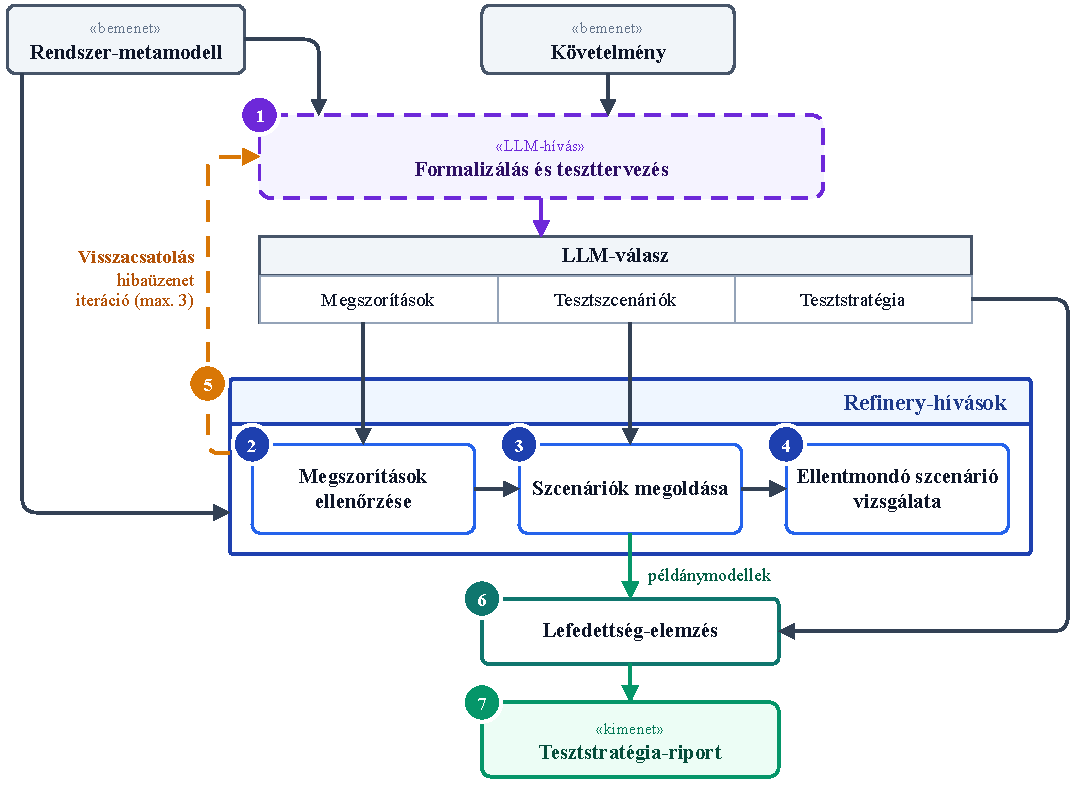
\includegraphics[width=\textwidth]{figures/overview-architecture.pdf}
	\caption{A megközelítés áttekintése. A számok a szövegben hivatkozott elemeket jelölik.}
	\label{fig:overview}
\end{figure}

Az ábrán a szaggatott lila keret az LLM-hívást, a kék sáv a Refinery-hívásokat, a narancssárga szaggatott nyíl a visszacsatolást jelöli. A megközelítés elemei a következők.

\begin{description}
	\item[Bemenetek.] A \emph{rendszer-metamodell} a rendszer formális modellje a Refinery modellezési nyelvén: leírja a rendszer elemeinek típusait és kapcsolatait, a rendszer rögzített, konkrét elemeit, valamint a rendszer már formalizált szabályait. A \emph{követelmény} egyetlen, természetes nyelven megfogalmazott rendszerkövetelmény, amelyhez a tesztstratégia készül.
	\item[\elem{1} Formalizálás és teszttervezés.] Egyetlen LLM-hívás, amely a követelményt és a metamodellt kapja meg, és háromrészes választ ad:
	\begin{itemize}
		\item \emph{megszorítások}: a követelmény formalizálása a metamodell fogalmaival, új gráfpredikátumok és hibapredikátumok formájában, amelyek a metamodellt kiegészítik, de nem módosítják;
		\item \emph{tesztszcenáriók}: néhány ténnyel rögzített, konkrét bemeneti helyzetek, amelyek megjelölik, hogy mely feltételek teljesülnek bennük és melyek nem;
		\item \emph{tesztstratégia}: a követelmény atomi feltételei és elvárásai, valamint az ezeket összekötő szabályok.
	\end{itemize}
	\item[\elem{2} Megszorítások ellenőrzése.] Refinery-hívás, amely a metamodellt és a generált megszorításokat együtt tölti be, és ellenőrzi, hogy a megszorítások szintaktikailag helyesek, csak létező típusokra és kapcsolatokra hivatkoznak, és csak kiegészítik a metamodellt.
	\item[\elem{3} Szcenáriók megoldása.] Minden tesztszcenárióra külön Refinery-hívás, amely a metamodell, a megszorítások és a szcenárió tényei alapján példánymodelleket generál, vagy megállapítja, hogy a szcenárió ellentmondásos.
	\item[\elem{4} Ellentmondó szcenárió vizsgálata.] Ellentmondásos szcenárió esetén egy újabb Refinery-hívás eldönti, hogy a helyzet már a metamodell szerkezete alapján is lehetetlen-e. A szerkezetileg lehetetlen negatív esetek kizárásra kerülnek, minden más ellentmondásos szcenárió elutasításra.
	\item[\elem{5} Visszacsatolás.] Ha a válasz bármely ellenőrzésen elbukik, a hibaüzenet visszakerül az LLM-hez, amely új választ ad. A ciklus legfeljebb három kísérletig ismétlődik.
	\item[\elem{6} Lefedettség-elemzés.] Az elfogadott válaszból döntési tábla készül arról, hogy melyik szcenárióban mely feltételek teljesülnek, mely szabályok aktiválódnak és mely elvárások kötelezők. Ebből látszik, hogy a szcenáriók a stratégia minden elemét tesztelik-e, és hol vannak hiányok.
	\item[\elem{7} Tesztstratégia-riport.] A kimenet: a mérnök által átnézhető dokumentum, amely a tesztstratégiát, a megszorításokat, a szcenáriókat példánymodellekkel, a lefedettség-elemzést és a validáció előzményeit tartalmazza.
\end{description}


%----------------------------------------------------------------------------
\section{Futó példa}
\label{sec:overview-example}
%----------------------------------------------------------------------------

A megközelítést egy ipari probléma által ihletett vasúti esettanulmányon mutatjuk be, amelynek metamodellje egy vonat fedélzeti rendszerét írja le. A vonathoz pontosan egy aktuális vonatesemény tartozik: érkezés (\texttt{Arrival}), indulás (\texttt{Departure}) vagy vészfékezés (\texttt{EmergencyStop}). Az esemény a vonat állapotát is tartalmazza: a sebességet, a megállási ablakhoz viszonyított helyzetet és az ajtók állapotát. A fedélzeti komponensek -- köztük a vonatkezelő komponens (TMC), az utastájékoztató komponens (PIC) és a kezelőképernyő -- egy-egy porton keresztül kapnak üzeneteket (a metamodellben \emph{bubble}); azt, hogy egy port mely üzeneteket kapja, az \texttt{allowedBubbles} kapcsolat adja meg. A közel 500 soros metamodell futó példához szükséges részletét \aref{lst:overview-metamodel}.~lista mutatja. Ebből látható például, hogy érkezéskor az ajtók szükségszerűen nyitva vannak, hiszen az érkezés pontosan egy \texttt{DoorsOpen} ajtóállapotot tartalmaz.

\begin{lstlisting}[language=refinery,float=ht,caption={A metamodell futó példához szükséges részlete.},label=lst:overview-metamodel]
class Train {
    contains Event[1] trainEvent
    % ...
}
abstract class Event.
class Arrival extends Event {
    contains ZeroSpeed[1] arrSpeed
    contains WithinStoppingWindow[1] arrWindow
    contains DoorsOpen[1] arrDoors
}
abstract class DoorState.
class DoorsOpen extends DoorState.
class DoorsClosed extends DoorState.
abstract class Component {
    contains Port[1] ComponentPorts opposite parent
}
class PassengerInformationComponent extends Component.
class Port {
    Bubble[] allowedBubbles
    % ...
}
class ArrivalEvent extends EventBubble.
pred isTargetPic(Port p) <->
    PassengerInformationComponent(pic), ComponentPorts(pic, p).
pred hasArrivalEvent(Port p) <->
    allowedBubbles(p, b), ArrivalEvent(b).
\end{lstlisting}

A futó példa követelménye a következő:
\begin{quote}
	\emph{IF the train event is Arrival AND the doors are DoorsOpen THEN the PassengerInformationComponent must receive an ArrivalEvent via PICPort.}
\end{quote}
Magyarul: ha a vonatesemény érkezés, és az ajtók nyitva vannak, akkor az utastájékoztató komponensnek a \texttt{PICPort} porton keresztül meg kell kapnia az \texttt{ArrivalEvent} üzenetet.


%----------------------------------------------------------------------------
\section{Formalizálás és teszttervezés}
\label{sec:overview-llm}
%----------------------------------------------------------------------------

Az \elem{1} LLM-hívás a követelményt és a teljes metamodellt kapja meg, egy rögzített utasításkészlettel együtt, amely a válasz szerkezetét és a Refinery nyelv szabályait írja le. A válasz három része egymásra hivatkozik: a szcenáriók a stratégia feltételeit jelölik meg, a stratégia szabályai pedig a feltételeket kötik össze az elvárásokkal.

\paragraph{Tesztstratégia.} A stratégia a követelményt atomi feltételekre és elvárásokra bontja. A feltételek a rendszer bemeneteire és állapotára, az elvárások a rendszer kimeneteire vonatkoznak; a szabályok azt adják meg, hogy a feltételek mely kombinációja mely elvárásokat teszi kötelezővé. Minden feltétel és elvárás megadja a követelmény szövegének azt a részét is, amelyből származik; ez a forrásszöveg teszi visszavezethetővé a stratégia elemeit a követelményre. A futó példa stratégiáját \aref{tab:overview-strategy}.~táblázat mutatja.

\begin{table}[!ht]
	\footnotesize
	\centering
	\begin{tabular}{l >{\raggedright\arraybackslash}p{0.36\textwidth} >{\raggedright\arraybackslash}p{0.42\textwidth}}
		\toprule
		Azonosító & Leírás & Forrásszöveg \\
		\midrule
		C1 & Az aktuális vonatesemény érkezés. & \emph{IF the train event is Arrival} \\
		C2 & Az eseményhez tartozó ajtóállapot nyitott. & \emph{AND the doors are DoorsOpen} \\
		E1 & A PIC a \texttt{PICPort} porton megkapja az \texttt{ArrivalEvent} üzenetet. & \emph{THEN the PassengerInformationComponent must receive an ArrivalEvent via PICPort} \\
		R1 & Ha C1 és C2 teljesül, akkor E1 kötelező. & -- \\
		\bottomrule
	\end{tabular}
	\caption{A futó példa tesztstratégiája: feltételek (C), elvárás (E) és szabály (R). A leírások az LLM angol nyelvű kimenetének fordításai.}
	\label{tab:overview-strategy}
\end{table}

\paragraph{Megszorítások.} A megszorítások a követelményt a metamodell fogalmaival formalizálják. A gráfpredikátumok (\texttt{pred}) a követelményben szereplő helyzeteket írják le, a hibapredikátumok (\texttt{error}) pedig a követelményt sértő állapotokat; egy érvényes példánymodellben egyetlen hibapredikátum sem teljesülhet. Minden új név \texttt{gen\_} előtagot kap, így a generált elemek elkülönülnek a metamodell elemeitől. A futó példában (\aref{lst:overview-constraints}.~lista) a \texttt{gen\_arrivalWithOpenDoors} predikátum a C1 és a C2 feltétel együttes teljesülését írja le, a \texttt{gen\_picMissingArrivalEvent} hibapredikátum pedig kizárja azokat az állapotokat, amelyekben ilyenkor a PIC portja nem kapja meg az \texttt{ArrivalEvent} üzenetet.

\begin{lstlisting}[language=refinery,float=ht,caption={A futó példa elfogadott megszorításai.},label=lst:overview-constraints]
pred gen_arrivalWithOpenDoors(Train t) <->
    trainEvent(t, e), Arrival(e), arrDoors(e, d), DoorsOpen(d).

error gen_picMissingArrivalEvent(Train t, Port p) <->
    gen_arrivalWithOpenDoors(t), isTargetPic(p), !hasArrivalEvent(p).
\end{lstlisting}

\paragraph{Tesztszcenáriók.} Egy szcenárió néhány ténnyel rögzít egy bemeneti helyzetet, és megjelöli, mely feltételek teljesülnek benne (például C1) és melyek nem (például $\neg$C1). A szcenárió csak a bemenetet rögzíti, a követelmény által elvárt kimenetet nem: azt a Refinery vezeti le (\aref{sec:overview-validation}.~szakasz). Azokat a szcenáriókat, amelyekben legalább egy feltétel jelölten nem teljesül, negatív eseteknek nevezzük. A futó példában az LLM négy szcenáriót tervezett: a TS1 pozitív esetben a vonat nyitott ajtókkal érkezik, a TS2-ben zárt ajtókkal indul, a TS3-ban peronnál, nyitott ajtókkal vészfékez, a TS4-ben pedig nyílt pályán, zárt ajtókkal vészfékez. A TS1 tényeit \aref{lst:overview-ts1}.~lista mutatja.


%----------------------------------------------------------------------------
\section{Ellenőrzés és visszacsatolás}
\label{sec:overview-validation}
%----------------------------------------------------------------------------

\Aref{fig:overview-validation}.~ábra az LLM-válasz ellenőrzését részletezi. A \elem{2} Refinery-hívás a metamodellt és a megszorításokat együtt tölti be. A válasz hibás, ha a megszorítások szintaktikailag hibásak, nem létező típusra vagy kapcsolatra hivatkoznak, vagy a predikátumokon kívül mást is tartalmaznak, például új osztályt vagy tényt, ami a metamodell módosítását jelentené.

\begin{figure}[!ht]
	\centering
	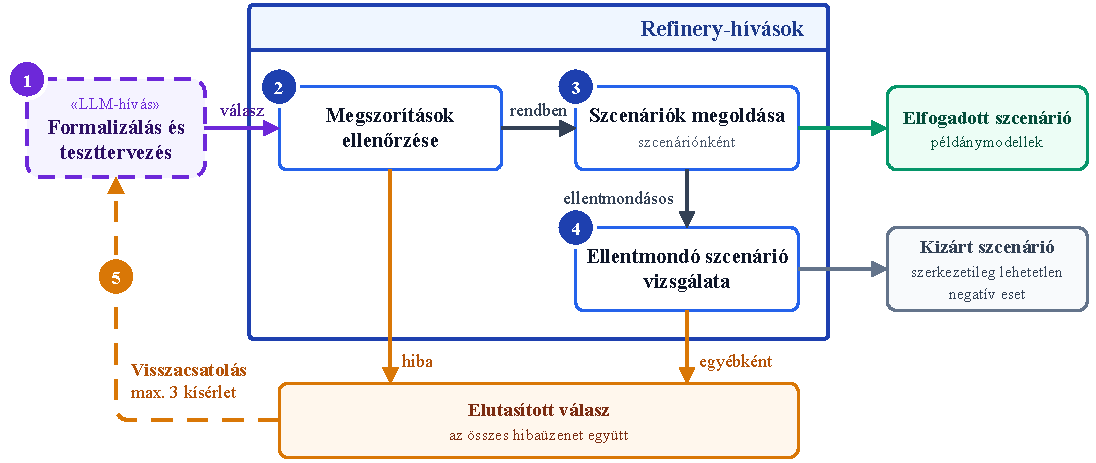
\includegraphics[width=\textwidth]{figures/overview-validation.pdf}
	\caption{Az LLM-válasz ellenőrzése és a visszacsatolás. A (3) és a (4) lépés minden szcenárióra lefut; a válasz akkor elfogadott, ha egyik szcenáriója sem elutasított.}
	\label{fig:overview-validation}
\end{figure}

A \elem{3} lépés minden szcenárióra külön modellgenerálást végez: a Refinery a metamodellből, a megszorításokból és a szcenárió tényeiből kiindulva legfeljebb tíz példánymodellt keres. A példánymodell a rendszer egy teljes, konkrét állapota, amelyben a metamodell szabályai és a generált megszorítások is teljesülnek. Ha van ilyen modell, a szcenárió elfogadott, és a modellek megmutatják, hogyan kell viselkednie a rendszernek az adott helyzetben. \Aref{lst:overview-ts1}.~lista a TS1 egyik példánymodelljének részletét is tartalmazza: a modellben a \texttt{PICPort} megkapja az \texttt{ArrivalEvent} üzenetet, vagyis az E1 elvárás teljesül, pedig ezt a kimenetet a szcenárió nem rögzítette. Az üzenet a TMC és a kezelőképernyő portjára is eljut, mert ezt a metamodell meglévő szabályai írják elő.

\begin{lstlisting}[language=refinery,float=ht,caption={A TS1 szcenárió bemeneti tényei és egy generált példánymodelljének részlete.},label=lst:overview-ts1]
% input facts of TS1
Arrival(obj1). trainEvent(t1, obj1).
DoorsOpen(obj2). arrDoors(obj1, obj2).

% excerpt of an instance model generated by Refinery (1 of 10)
ArrivalEvent(arrivalEvent1).
allowedBubbles(PICPort, arrivalEvent1).
allowedBubbles(TMCPort, arrivalEvent1).
allowedBubbles(screenPort, arrivalEvent1).
ZeroSpeed(zeroSpeed1). arrSpeed(obj1, zeroSpeed1).
\end{lstlisting}

Ha egy szcenárióhoz nem létezik példánymodell, a szcenárió ellentmondásos. Ennek két oka lehet: vagy a helyzet a valóságban sem fordulhat elő, vagy a válasz hibás, például mert a megszorítások túl szigorúak. A \elem{4} Refinery-hívás ezt úgy dönti el, hogy a szcenáriót csak a metamodell szerkezetével -- a típusokkal, a tartalmazási kapcsolatokkal és a multiplicitásokkal --, a szabályok és a megszorítások nélkül vizsgálja. Ha a helyzet már szerkezetileg is lehetetlen, és a szcenárió negatív esetnek készült, akkor a szcenárió kizárásra kerül, hiszen ilyen bemenet a rendszerben nem állhat elő. Ha például az LLM a C2 feltétel negatív esetét érkezéssel és zárt ajtókkal írná le, ez a szcenárió kizárásra kerülne, mert a metamodellben az érkezés mindig nyitott ajtóállapotot tartalmaz (\aref{lst:overview-metamodel}.~lista). Minden más ellentmondásos szcenárió elutasításra kerül.

A válasz elutasított, ha a megszorítások hibásak, ha legalább egy szcenárió elutasításra került, vagy ha egyetlen szcenárió sem elfogadott. Ekkor az \elem{5} visszacsatolás az összes hibaüzenetet egyszerre visszaküldi az LLM-nek, amely új, teljes választ ad. A ciklus legfeljebb három kísérletig tart; ha egyik válasz sem érvényes, a megközelítés nem ad ki tesztstratégiát.

A futó példában az LLM első válaszának megszorításai a követelményen túlmenő tiltást is tartalmaztak: érkezéskor az \texttt{ArrivalEvent} üzenet a PIC portján kívül más célporton nem jelenhetett meg. A metamodell szabályai szerint azonban érkezéskor ez az üzenet a TMC és a kezelőképernyő portjára is eljut, ezért az első válasz minden olyan szcenáriója ellentmondásos lett, amelyben a vonat nyitott ajtókkal érkezik. Mivel ezek a helyzetek szerkezetileg lehetségesek, a Refinery mindhárom ilyen szcenáriót elutasította, és a következő hibaüzenet került vissza az LLM-hez:
\begin{quote}
	\raggedright\small\texttt{Test scenario TS1 is UNSATISFIABLE. Test scenario TS2 is UNSATISFIABLE. Test scenario TS4 is UNSATISFIABLE.}
\end{quote}
A második válasz már csak a követelményben szereplő elvárást formalizálta (\aref{lst:overview-constraints}.~lista), és mind a négy szcenáriója elfogadott lett.


%----------------------------------------------------------------------------
\section{Lefedettség-elemzés és riport}
\label{sec:overview-coverage}
%----------------------------------------------------------------------------

A \elem{6} lefedettség-elemzés az elfogadott válasz tesztstratégiájából és szcenárióiból döntési táblát készít (\aref{tab:overview-decision}.~táblázat). A tábla minden elfogadott szcenárióhoz megadja a feltételek értékét, az aktiválódó szabályokat -- vagyis azokat, amelyek feltétele ezekkel az értékekkel igaz --, az általuk megkövetelt elvárásokat, valamint a példánymodellek számát. A feltételek értékei a szcenáriók jelöléseiből származnak; a Refinery azt garantálja, hogy minden elfogadott szcenárió a rendszer egy lehetséges állapota.

\begin{table}[!ht]
	\footnotesize
	\centering
	\begin{tabular}{l >{\raggedright\arraybackslash}p{0.36\textwidth} c c c c r}
		\toprule
		Szcenárió & Bemeneti helyzet & C1 & C2 & Szabály & Elvárás & Modellek \\
		\midrule
		TS1 & érkezés, nyitott ajtók & I & I & R1 & E1 & 10 \\
		TS2 & indulás, zárt ajtók & H & H & -- & -- & 4 \\
		TS3 & vészfékezés peronnál, nyitott ajtók & H & I & -- & -- & 10 \\
		TS4 & vészfékezés nyílt pályán, zárt ajtók & H & H & -- & -- & 8 \\
		\bottomrule
	\end{tabular}
	\caption{A futó példa döntési táblája. I: a feltétel teljesül, H: nem teljesül; Szabály: az aktiválódó szabályok; Elvárás: az általuk megkövetelt elvárások.}
	\label{tab:overview-decision}
\end{table}

A döntési táblából három lefedettségi kritérium számítható: minden feltétel legalább egy szcenárióban teljesüljön és legalább egyben ne; minden szabály legalább egy szcenárióban aktiválódjon és legalább egyben ne; minden elvárást legalább egy szcenárió követeljen meg. A futó példában mindhárom kritérium teljesül: a C2 például a TS1-ben és a TS3-ban teljesül, a TS2-ben és a TS4-ben nem, az R1 szabály pedig csak a TS1-ben aktiválódik, így az E1 elvárást a TS1 követeli meg. Ha egy elem nem teljesíti a kritériumot, vagy a stratégia hiányos -- például egy szabály nem deklarált feltételre hivatkozik --, az elemzés ezt hiányként jelzi.

A \elem{7} tesztstratégia-riport a mérnök számára átnézhető dokumentum. Tartalmazza a követelményt, a tesztstratégiát a forrásszövegekkel, a generált megszorításokat, a szcenáriókat a tényeikkel és egy-egy példánymodellel, a kizárt szcenáriókat, a lefedettség-elemzést, valamint a validáció előzményeit, vagyis az elutasított kísérleteket és a hozzájuk tartozó hibaüzeneteket. A riport elemei azonosítóval hivatkoznak egymásra, így a szcenáriók, a szabályok, a feltételek és az elvárások a forrásszövegen keresztül visszavezethetők a követelményre. A futó példa riportja azt is rögzíti, hogy a stratégiát a Refinery a második kísérletben fogadta el.
